\section{Introduction}

Reinforcement learning algorithms generally belong to one of two categories: model-based techniques, which attempt to overcome the issue of a lack of prior knowledge by enabling the agent to construct a representation of its environment, and model-free techniques, which learn a direct mapping from states to actions. Model-free approaches are typically less practical because running a simulation is very time consuming or expensive, and model-based approaches tend to achieve lower asymptotic performance due to the error in model approximation. To design an effective model-based algorithm, Janner, M. et al \cite{ref1}. studies the role of model usage in policy optimization and introduces a practical algorithm called model-based policy optimization (MBPO), which makes limited use of a predictive model to achieve pronounced improvements in performance comparing to other model-based approaches.

The authors of the paper \cite{ref1} first formulate and analyze a general implementation for MBPO with monotonic improvement at each step which uses a predictive model to optimize policy and utilizes the policy to collect data and train the model. Previous study shows it is difficult to justify model usage due to pessimistic bounds on model error and this paper finds a way to modify the pessimistic bounds which solves the problem. Based on the analysis, the authors propose a simple model-based reinforcement learning algorithm of using short model-generated rollouts branched from real data to improve model effectiveness. The experiments show this algorithm is faster than other state-of-the-art model-based methods such as STEVE \cite{ref2}, and matches the performance of the best model-free methods like SAC \cite{ref3}.

In this reproducibility report, we study in detail the MBPO algorithm described in the paper (detailed in Section 3). Our work mainly focuses on the replication of their algorithm and the re-implementation of their predictive model but in a PyTorch version (detailed in Section 4). Lastly, we describe our experiments and provide insightful analysis of our results (detailed in Section 5). We provide the source code\footnote{\url{https://github.com/jxu43/replication-mbpo}} for generating the results and setting up the experiments.

\section{Target Questions}
In order to assess the reproducibility of the paper and validate its conclusions, the main questions we will focus on are:
\begin{itemize}
    \item Can we validate the performance of MBPO on two different benchmarks \cite{ref4} (Hopper and Walker2d)?
    \item Compared to different baselines, can MBPO achieve a pronounced better performance than these model-based and model-free algorithms?
    \item How the proposed MBPO algorithm can be further improved?
\end{itemize}

\section{Methodology}

\subsection{Overview}
This section introduces the details of the paper's theory and approaches. The main contribution of the paper is to introduce the MBPO algorithm which resolves the problem that accompanies during monotonic model-based improvement when the model error $\epsilon_m$ is high. Specifically, instead of propagating the predictive model for long trajectories, the authors suggest a method of disentangling the task horizon and the model propagation horizon \cite{ref5}. The method chooses the random states observed previously during interaction with the environment and propagates short trajectories forward. The authors propose that this approach would effectively reduce the effect of compounding errors, and make policy learning substantially faster than most model-based ones while retaining the quality of the policy. To accomplish this goal, the main implementation is divided into three parts: a ensemble of probabilistic neural network, a policy optimizer, and the MBPO algorithm. The implementation of MBPO of the original paper is described in Algorithm 1.

\begin{algorithm}
\caption{Model-Based Policy Optimization with Deep Reinforcement Learning}\label{euclid}
\begin{algorithmic}[1]
\State Initialize policy $\pi_{\phi}$, predictive model $p_{\theta}$, environment dataset $D_{env}$, model dataset $D_{model}$
\For{N epochs}
\State Train model $p_{\theta}$ on $D_{env}$ via maximum likelihood
\For{E steps}
\State Take action in environment according to $\pi_{\phi}$; add to $D_{env}$
\For{M model rollouts}
\State Sample $s_{t}$ uniformly from $D_{env}$
\State Perform k-step model rollout starting from $s_{t}$ using $\pi_{\phi}$; add to $D_{model}$
\EndFor
\For{G gradient updates}
\State Update policy parameters on model data: $\phi \leftarrow \phi - \lambda_{\pi} \hat{\Delta} J_{\pi}(\pi, D_{model})$
\EndFor
\EndFor
\EndFor
\end{algorithmic}
\end{algorithm}

\subsection{Predictive Model}

The authors use the ensemble of probabilistic neural networks from the PETS \cite{ref6}. It is a bootstrap ensemble of dynamics models. Each member of the ensemble has an output that parametrizes a Gaussian distribution. To generate a prediction from the ensemble, the authors randomly choose a model, so that different dynamics models can sample different transitions along a single model rollout. Predictive models are preferable because they combine the sample efficiency of a model-based approach with the asymptotic performance of function approximators \cite{ref7}.

\subsection{Soft Actor-Critic for Policy Optimization}

The authors choose Haarnoja's soft-actor critic algorithm (SAC), which is an off-policy model free deep RL algorithm, as the policy optimization algorithm. The most critical feature of this algorithm is entropy regularization, which is used to maximize expected reward while also maximize entropy. 
SAC concurrently learns a policy $\pi_{\theta}$, two Q-functions $Q_{\phi 1}$, $Q_{\phi 2}$ and a value function $V_{\psi}$. It considers the entropy augmented objective:
$$J(\pi) = E_{\pi} \left[\sum_{t}r(s_{t},a_{t}) - \alpha log(\pi(a_{t}|s_{t}))\right]$$
Since the objective function consists of both a reward term and an entropy term, SAC encourages the policy network to explore and not assign a very high probability to any one of the actions. It controls the trade-off between exploration and exploitation by using a temperature parameter to determine the relative importance of the entropy term against the reward. SAC provides us a substantial improvement in exploration and robustness as maximum entropy policies could improve exploration by exploring diverse behaviors and reduces estimation errors \cite{ref8}. Furthermore, as SAC is an off-policy method, it can reuse data collected for another task and will not suffer from poor sample complexity. Generally, the idea is that learned models may be incorporated into model-free methods for improvements in data
efficiency.

\subsection{Model-Based Policy Optimization}

The authors state a way of optimization which interpolates model-based and model-free updates. It chooses to rely less on the model and instead more on real data collected from the true dynamics when the model is inaccurate. To achieve that, performing rollout is a desirable approach. In order to allow for dynamic adjustment between model-based and model-free rollouts, the authors introduce the notion of a \textit{branched rollout}, in which they begin a rollout from a state under the previous state distribution of the real environment dataset and run k steps according to $\pi$ under the predictive model $p_{\theta}$. Under the k-branched rollout method, using model error under the updated policy $\epsilon_{m'}$, the equation of rollouts can be bounded into the following equation:
$$
    \eta[\pi] \geq \eta^{branch}[\pi] - 2r_{max}[\frac{\gamma^{k+1}\epsilon_{\pi}}{(1-\gamma)^2} + \frac{\gamma^{k}\epsilon_{\pi}}{(1-\gamma)} + \frac{k}{1-\gamma}(\epsilon_{m'})]
$$
The bound above motivates the authors' MBPO algorithm, which makes limited use of truncated, but nonzero-length, model rollouts.\\

\begin{figure}[h]
  \centering
  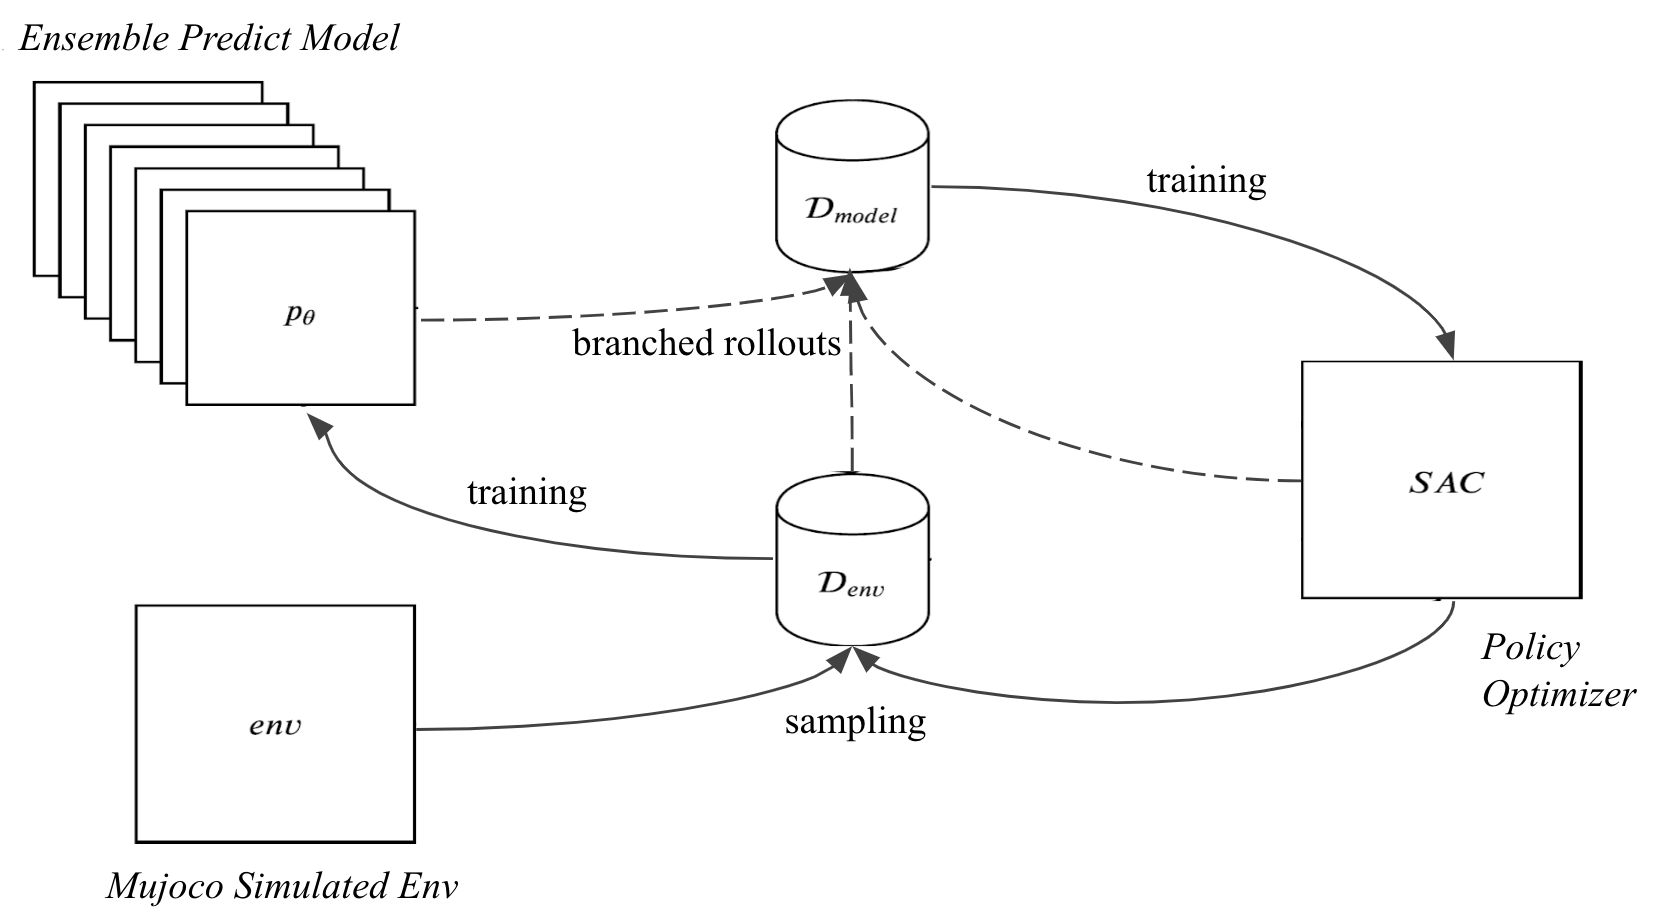
\includegraphics[width=10cm]{../openreview/mbpo_new.png}
  \caption{Diagram of Algorithm Pseudocode.}
\end{figure}

Figure 1 above is the diagram of the paper's algorithm. For each epoch, the authors train the predictive model from the samples of environment dataset $D_{env}$, and during each step in the epoch, they suggest to interact with the environments with the current policy from SAC, and add the state-action pairs to $D_{env}$. Then there will be M number of rollout. Each rollout is consist of choosing a random state from $D_{env}$ at each time step, and applying the policy generated from SAC algorithm to perform the rollout. After that, they use the generated data to optimize the policy using SAC as the policy optimization algorithm. Using the approach above, the authors claim to achieve the results that are more effective than the best model-free algorithms, and surpass some recent model-based methods such as PETS.

\section{Reproducibility}
This section will introduce the details of our re-implementation. The main contribution of the original paper is the MBPO algorithm, and we fully re-implemented the MBPO based on both the algorithm and hyperparameters of the original paper and the public codes of the original paper. We followed the codes here because some details are missing in the description of the algorithm in the original paper, which will be discussed extensively in the following parts. For the predictive model, the authors of the original paper uses the existing implementation of PETS by TensorFlow, however, we also re-implemented this part with PyTorch. We experimented with both PETS and our reproduced predictive model by PyTorch. For the policy, the original paper leverage the existing implementation of Softlearning by TensorFlow, while we chose to use another existing implementation of SAC by PyTorch.

%\subsection*{Implementation}
\subsection{Predictive Model}
The authors use an existing bootstrap ensemble model PETS as the predictive model and each single model is a multi-layer fully connected neural network which whose outputs parametrize a Gaussian distribution. In order to generate a prediction from the ensemble model, the algorithm will select a single model randomly from the top n models with minimum loss. We re-implement the predictive model by PyTorch with the same structure, however due to the difference between PyTorch and TensorFlow, we have to make some changes to accomplish the same functionalities like how to generate an ensemble model. We experiment with both the PETS and our re-implemented predictive model. The results will be discussed in the next section.

\subsection{Soft Actor-Critic for policy optimization}
The authors used the existing reinforcement learning framework "Softlearning" which includes the official implementation of the Soft Actor-Critic algorithm. This toolbox trains maximum entropy policies in continuous domains and utilizes the TensorFlow modules for their models. Instead of using their entire framework, we use a PyTorch implementation of SAC to provide policy optimization \cite{ref9}. We experiment with the efficiency and performance of the PyTorch implementation and the results are convincing. Since we are able to reproduce results by using the PyTorch SAC and it is much easier to integrate it with the rest piece of our MBPO, we decide to use the PyTorch implementation.

\subsection{Model-Based Policy Optimization(MBPO) with Deep Reinforcement Learning}

The MBPO algorithm is the main contribution of the original paper, thus we put more efforts into fully re-implementing the MBPO algorithm and experimenting with different environments. Generally we followed the same procedure as the algorithm in the original paper. The Algorithm 1 above is the pseudocode for the algorithm described in the original paper, and Algorithm 2 is our detailed algorithm to re-implement the MBPO algorithm, which shows more details about the parameters and algorithm itself. 

\begin{algorithm}
\caption{Re-implemented Model-Based Policy Optimization with Deep Reinforcement Learning}\label{euclid}
\begin{algorithmic}[1]
\State Initialize policy $\pi_{\phi}$, predictive model $p_{\theta}$, environment dataset $D_{env}$, model dataset $D_{model}$
\For{T steps}
\State Take action in environment according to initial policy $\pi_{\phi}$; add to $D_{env}$
\EndFor
\For{N epochs}
\For{E steps}
\State Train model $p_{\theta}$ on $D_{env}$ per F steps
\State Take action in environment according to $\pi_{\phi}$; add to $D_{env}$
\For{M model rollouts}
\State Sample $s_{t}$ uniformly from $D_{env}$
\State Perform k-step model rollout starting from $s_{t}$ using $\pi_{\phi}$; add to $D_{model}$
\EndFor
\For{G gradient updates}
\State Update policy parameters on model data and environment data with a ratio of $(1 - r) : r$: $\phi \leftarrow \phi - \lambda_{\pi} \hat{\Delta} J_{\pi}(\pi, [D_{model}, D_{env}])$
\EndFor
\EndFor
\EndFor
\end{algorithmic}
\end{algorithm}

Firstly, there are T steps sampling in real environment with initial policy $\pi_{\phi}$ before the following training process. As the policy has not been trained at this time, the current actions will be totally random choices, which means that these sampling steps will be exploration steps. These steps are important for the following rollouts because those rollouts will start from the samples uniformly randomly chosen from the environment dataset. Secondly, MBPO may train the predictive model once per F steps rather than training the model only once per epoch. It is designed to train the model more frequently so that the rollouts from the predictive model will be more accurate. There will be M rollouts in each step and there will be E steps per epoch, thus when E is set to be a large number, training the predictive model only once per epoch may be not sufficient for a complex environment. For Hopper and Walker2d, the predictive model will be trained once per 250 steps. Then the policy will not be updated only by the data sampled by the predictive model. A small portion of data sampled from the real environment will also be used to update the policy. It helps to update the policy more accurately especially when the predictive model has not been trained well at the beginning. As described in the appendix of the original paper, the rollout length k may be changed dynamically along with the growth of epochs with the equation $k = min(max(x + \frac{e-a}{b-a}(y-x), x), y)$, where e is the current epoch number, a and b are the minimum epoch and maximum epoch respectively, and x and y are the minimum rollout length and maximum rollout length respectively. 

\subsection{Reproducibility Costs}
Given that there was no mention in the paper about computational resources required, we describe the computational cost for running the experiments. All of our experiments are conducted on Google Cloud Platform. We use NVIDIA Tesla P100 GPU for each experiment, and we replicate three baselines to make comparisons, which are SAC, SLBO \cite{ref10}, and STEVE. We implement two versions of predictive models, one in TensorFlow, another in Pytorch. They both take seven hours to run 150k steps. SAC takes about one hour for training 150k steps which is much faster than other baselines since it is a model-free algorithm and no need to train model. SLBO takes around eight hours while STEVE takes 20 hours to train 150k steps. In conclusion, model-based methods usually take much longer than model-free methods and they need much more computational costs. Our reproducibility needs relatively large costs in terms of time and computing resources.

\section{Results and Analysis}
\begin{table}[h]
  \caption{Hyperparameter Settings}
  \centering
  \begin{tabular}{cccc}
    \toprule
    \cmidrule(r){0-3}
        & Description     & Hopper         & Walker2d   \\
    \midrule
    N   & epoch           & 125               & 300           \\
    E   & environment steps per epoch & 1000               & 1000           \\
    M   & model rollouts per environment step       & 400      &    400           \\
    B   & ensemble size           & 7               & 7           \\
    G   & policy updates per environment step           & 20               & 20           \\ 
    k   & model horizon           &  1              & 1 -> 25 over epochs 20 -> 100           \\
    r   & real ratio           &  0.05             & 0.05           \\
    F   & train frequency for predictive model           &  250             & 250           \\
    T   & initial sampling steps for real environment          &  5000             & 5000           \\
    \bottomrule
  \end{tabular}
\end{table}
\subsection{Experiments Settings}

In our experiments, we aim to see if our replicated MBPO algorithm can yield similar experimental results in the paper and how well our algorithm performs in comparison to the best model-based and model-free reinforcement learning algorithms. For the model-based methods, we use STEVE and SLBO as baselines. STEVE is an extension to model-based value expansion (MVE) \cite{ref11}. Compared to MVE, it interpolates between many different horizon lengths, favoring those whose estimates have lower uncertainty, and thus lower error. SLBO achieves state-of-the-art performance when only one million or fewer samples are permitted on a range of continuous control benchmark tasks. For model-free methods, we choose SAC as our baseline since our model-based algorithm uses it for policy learning \& updating and this baseline can help us understand the difference of integrating a model. Comparisons with those state-of-the-art model-based and model-free methods validate the performance of our work.

Based on objective reasons such as time and computing resources, we evaluate our MBPO algorithm and above baselines on two MuJoCo-simulated benchmark environments which are Hopper and Walker2d. For each result graph, we use steps as our Horizontal axis and average return as our vertical axis to measure the performance of each baseline and compare our MBPO method with other baselines to see if it is much faster than other model-based algorithms and has asymptotic performance similar to the model-free algorithm.

Following the paper, our replicated algorithm used the same hyperparameter settings provided in the appendix of original paper with some parameters defined in the authors' public codes. Table 1 shows the parameters we used for the results we will present in the following subsections.

\subsection{MBPO Evaluation}
We evaluated our MBPO algorithm against the original MBPO on two benchmarks to verify whether the algorithm's performance can match the original paper.  
%insert images - 2 image (hopper + walker2d) + figure explanation!!!!! 
% \begin{figure}[h]
%   \centering
%   \fbox{\rule[-.5cm]{0cm}{2cm}\includegraphics[width =7cm]{compareToOriginHopper} \rule[-.5cm]{0cm}{2cm}\includegraphics[width = 7cm]{compareToOriginWalker2d}}
%   \caption{Original MBPO vs. replicated MBPO}
% \end{figure}

\begin{figure}[h]
\centering
\begin{minipage}[t]{0.48\textwidth}
\centering
\includegraphics[width=6cm]{../openreview/compareToOriginHopper}
\end{minipage}
\begin{minipage}[t]{0.48\textwidth}
\centering
\includegraphics[width=6cm]{../openreview/compareToOriginWalker2d}
\end{minipage}
\caption{Original MBPO vs. Replicated MBPO}
\end{figure}

%add hyperlink
Figure 2 is the learning curves of the two algorithms. The original MBPO's data is provided by the authors which is a combination of five trials. The replicated MBPO's data is a combination of three trials we ran. Solid curves depict the mean of the trials we ran and the shaded regions correspond to standard deviation among trials. Replicated MBPO has the similar performance to the paper results. Concisely, there is no major difference on average return after 75k steps on Hoppers and 10k steps on Walker2d. We evaluated two algorithms on the standard 1000-step versions of the benchmarks.

The Figure shows that our re-implemented MBPO can achieve comparable performance on both two benchmarks. Our method on Hopper can even attain higher rewards after convergence and it converges a little bit faster than the original one. Better reward is possibly related to the different version of policy optimizer SAC we used in our implementation. However, our results show greater fluctuation. The reason might be that we don't have enough  trials to take average so we have occasional outliers. 

\subsection{Baseline Evaluation}

In our comparison, we also aim to understand how well the reproduction of MBPO compares to the state-of-the-art model-based (STEVE, SLBO) and model-free (SAC) methods. We use the standard full-length version of the two tasks Hopper and Walker2d to conduct the experiments following the paper. 

\begin{figure}[h]
\centering
\begin{minipage}[t]{0.48\textwidth}
\centering
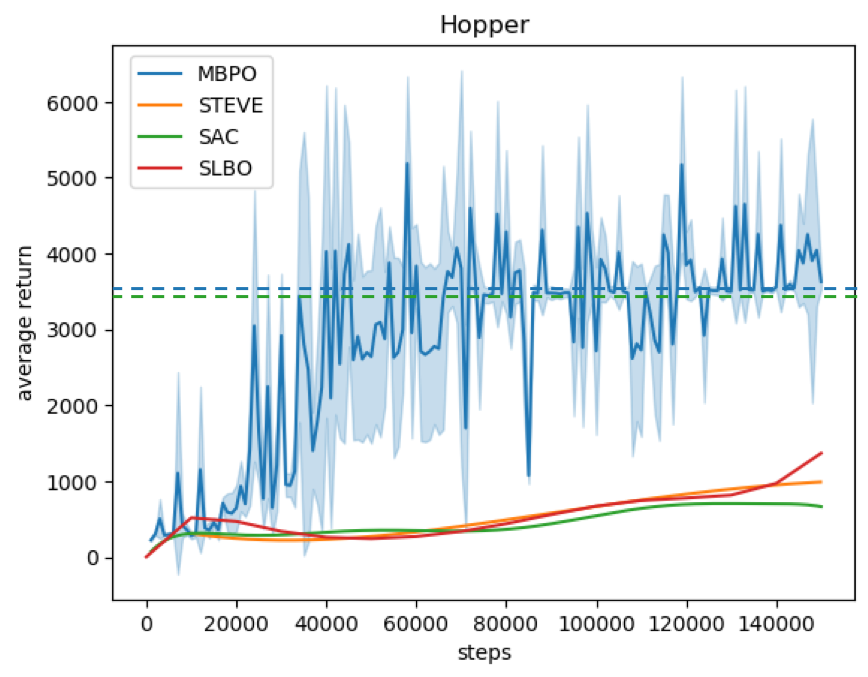
\includegraphics[width=6cm]{../openreview/Picture1.png}
\end{minipage}
\begin{minipage}[t]{0.48\textwidth}
\centering
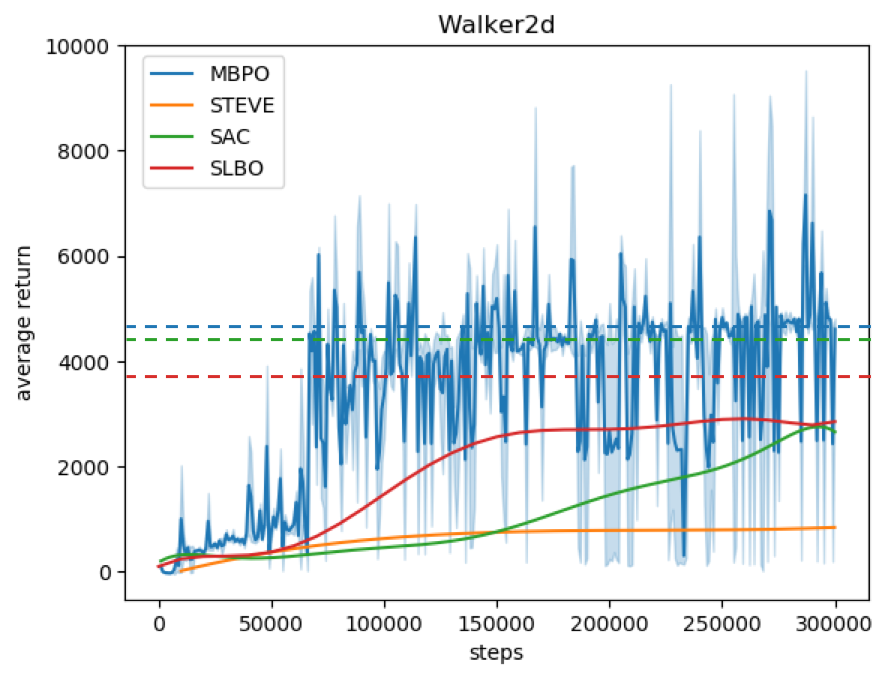
\includegraphics[width=6cm]{../openreview/Picture2.png}
\end{minipage}
\caption{Replicated MBPO vs. Baselines}
\end{figure}

Figure 3 shows the training curves of re-implemented MBPO and three baselines on different benchmarks. The blue solid line and shaded area are the mean and standard deviation of our MBPO experiments. The yellow, green and pink curves represent the fitted results of our one trial of the baselines. The dashed lines with different colors represents the average return on convergence of different algorithms. We may observe that MBPO does outperform on both two experiments. Specifically, MBPO learns substantially faster, an order of magnitude faster on Hopper, than prior methods, while attaining comparable or better final performance. For example, MBPO converges after 150k steps on Walker2d while model-free SAC converges after 650k steps with the approximately same average return. Also, MBPO converges at a higher average reward than model-based SLBO method. Thus, we may validate that the proposed MBPO algorithm has asymptotic performance rivaling the best model-free algorithms and learns substantially faster than prior model-free or model-based methods.

\subsection{Predictive Model Effects on Performance}

Seeking for improvements on the average rewards, we ran our MBPO using two different versions of predictive model which are the ensemble model from PETS in TensorFlow and our own ensemble model of 7 probabilistic neural networks in PyTorch. Figure 4 shows the results of the experiments.

\begin{figure}[h]
\centering
\begin{minipage}[t]{0.48\textwidth}
\centering
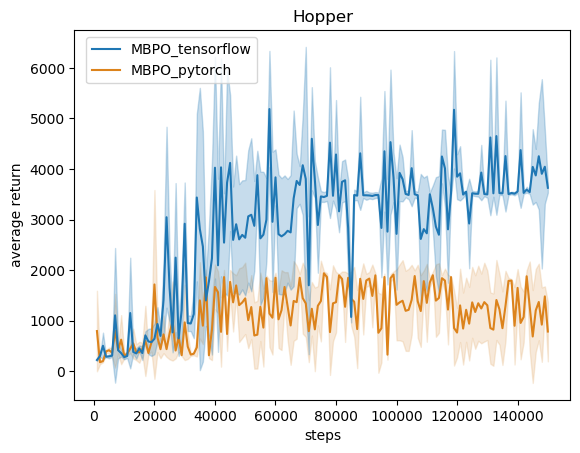
\includegraphics[width=6cm]{../openreview/tfVSpyHopper.png}
\end{minipage}
\begin{minipage}[t]{0.48\textwidth}
\centering
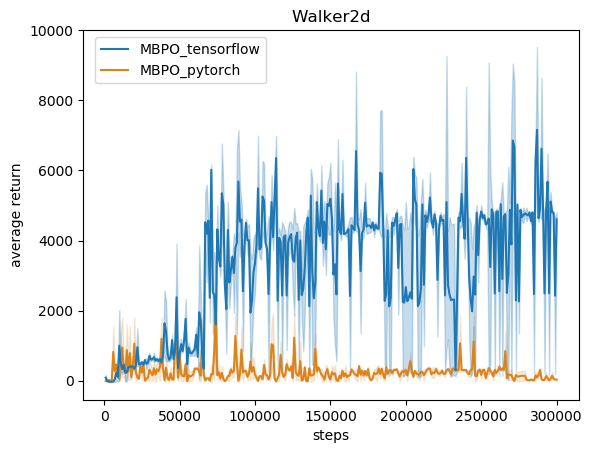
\includegraphics[width=6cm]{../openreview/tfVSpyWalker2d.png}
\end{minipage}
\caption{Predictive model in TensorFlow version vs. Predictive model in PyTorch version}
\end{figure}

Generally, the results with our re-implemented predictive model cannot compete with the results using the existing PETS model, especially on Walker2d. That is probably due to the difference between TensorFlow and PyTorch, and we do not have enough resources to tune our predictive model.

\subsection{Exploration on Hyper Parameters}

The algorithm described in the paper omits some details. Additionally, there are some differences between the algorithms pseudocode described in the paper and the real implementation by the authors. Specifically, the authors described the training update frequency as 1 per 1000 steps but implemented as 1 per 250 steps. Moreover, the pseudocode did not include any data sampled from the real environment during the policy training process. We decided to implement both algorithms and compare the results. Figure 5 shows the difference between these two settings, and demonstrates that the described algorithm in the paper will not generate the desired results as the paper shows.

\begin{figure}[h]
  \centering
  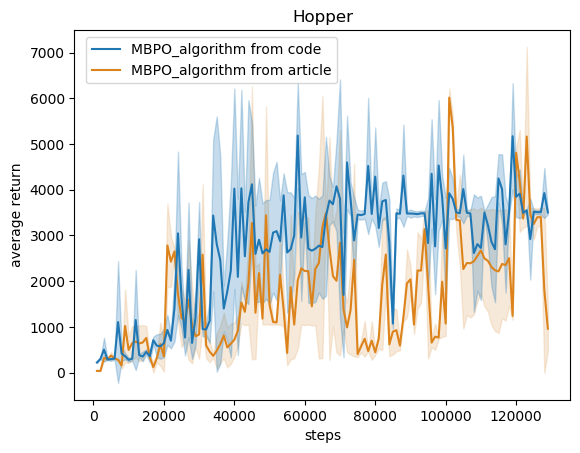
\includegraphics[width=8cm]{../openreview/paperVsCodeMBPO}
  \caption{MBPO follows the paper's algorithm vs. MBPO follows the authors' coding sequence}
\end{figure}

Due to the limitation of time and GCP credits, we cannot tune the hyperparameters thoroughly. The following is an example of our attempt to tune the rollout size M. The default rollout size M is 400 and we experimented on a rollout size 4000 to see whether a larger rollout size will lead to faster convergence. Figure 6 shows that the performance with rollout size 400 is quite similar to the performance with rollout size 4000.

\begin{figure}[h]
  \centering
  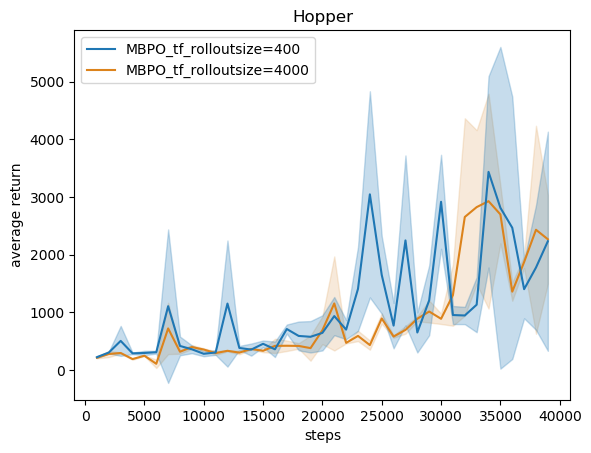
\includegraphics[width=8cm]{../openreview/differentRollOutSize}
  \caption{Our MBPO's performance with different rollout sizes}
\end{figure}

\section{Conclusion}
In summary, despite some inconsistencies between the pseudocode and real code as we discussed above, we have successfully reproduced the main results presented by Janner, M. et al., which confirms the supremacy of MBPO algorithm over other baseline models in variety of RL problems, e.g. STEVE and SAC. Due to limit of time, fewer repeats of our re-implemented model have been run. This could be the reason for the overall higher standard deviation in our results. However, the intense fluctuation of average return in our model comparing to the authors` results should demand a further research. Overall, we should applaud for the authors for providing such practical algorithm which not only guarantees the monotonic improvement at each step, but also prevents the error from accumulating by dynamically controlling the rollout length.

\section*{Acknowledgement}
To achieve this reproducibility challenge, we consulted some related materials other than paper itself, including the different versions of SAC implementations, the review of the paper. All the materials we consulted are included in the reference.
We want to thank all the staffs in Brown University CS2951-F, especially our professor Michael Littman, and our mentor TA Evan Cater for their help on clarifications and suggestions. Thank Google Cloud Platform for providing computational resources.

\newpage
\hypersetup{linkcolor=black,urlcolor=darkgray}
\renewcommand\emph[1]{{\bfseries #1}}
\setlength\bibitemsep{0pt}
\begin{thebibliography}{99}
\bibitem{ref1} Janner, M., Fu, J., Zhang, M., \& Levine, S. (2019). When to Trust Your Model: Model-Based Policy Optimization. arXiv preprint arXiv:1906.08253. 
\bibitem{ref2} Buckman, J., Hafner, D., Tucker, G., Brevdo, E., \& Lee, H. (2018). Sample-efficient reinforcement learning with stochastic ensemble value expansion. In Advances in Neural Information Processing Systems (pp. 8224-8234). 

\bibitem{ref3} Haarnoja, T., Zhou, A., Abbeel, P., \& Levine, S. (2018). Soft actor-critic: Off-policy maximum entropy deep reinforcement learning with a stochastic actor. arXiv preprint arXiv:1801.01290. 

\bibitem{ref4} Todorov, E., Erez, T., \& Tassa, Y. (2012, October). Mujoco: A physics engine for model-based control. In 2012 IEEE/RSJ International Conference on Intelligent Robots and Systems (pp. 5026-5033). IEEE. 

\bibitem{ref5} Or Rivlin. Model Based Policy Optimization {\small Reviewing recent advances in model-based reinforcement learning.}

\bibitem{ref6} Chua, K., Calandra, R., McAllister, R., \& Levine, S. (2018). Deep reinforcement learning in a handful of trials using probabilistic dynamics models. In Advances in Neural Information Processing Systems (pp. 4754-4765).

\bibitem{ref7} Nagabandi, A., Kahn, G., Fearing, R. S., \& Levine, S. (2018, May). Neural network dynamics for model-based deep reinforcement learning with model-free fine-tuning. In 2018 IEEE International Conference on Robotics and Automation (ICRA) (pp. 7559-7566). IEEE.

\bibitem{ref8} Haarnoja, T., Tang, H., Abbeel, P., \& Levine, S. (2017, August). Reinforcement learning with deep energy-based policies. In Proceedings of the 34th International Conference on Machine Learning-Volume 70 (pp. 1352-1361). JMLR. org.

\bibitem{ref9} Github: pytorch-soft-actor-critic. \url{https://github.com/pranz24/pytorch-soft-actor-critic}.

\bibitem{ref10} Luo, Y., Xu, H., Li, Y., Tian, Y., Darrell, T., \& Ma, T. (2018). Algorithmic framework for model-based deep reinforcement learning with theoretical guarantees. arXiv preprint arXiv:1807.03858.

\bibitem{ref11} Feinberg, V., Wan, A., Stoica, I., Jordan, M. I., Gonzalez, J. E., \& Levine, S. (2018). Model-based value estimation for efficient model-free reinforcement learning. arXiv preprint arXiv:1803.00101.
\end{thebibliography}

